\documentclass[12pt]{report}

\usepackage{amsmath}
\usepackage{pgfplots}
\usepgfplotslibrary{units}
\usepackage[russian]{babel}
\usepackage{filecontents}
\usepackage{titlesec, blindtext, color}
\usepackage{listings}

\usepackage{titlesec, blindtext, color} 
\definecolor{gray75}{gray}{0.75} 
\newcommand{\hsp}{\hspace{20pt}} 

\usepackage{geometry}
\geometry{top=0.5cm}


\lstset{ 
language=haskell,                 
basicstyle=\small\sffamily, 
numbers=left,              
numberstyle=\tiny,        
stepnumber=1,              
numbersep=5pt,             
showspaces=false,          
showstringspaces=false,   
showtabs=false,             
frame=single,            
tabsize=2,                
captionpos=t,              
breaklines=true,           
breakatwhitespace=false, 
escapeinside={\#*}{*)}   
}

\titleformat{\chapter}[hang]{\Huge\bfseries}{\thechapter\hsp\textcolor{gray75}{|}\hsp}{0pt}{\Huge\bfseries}

\begin{filecontents}{uMult.dat}
1000 0.0059538099999999995
1100 0.00650186
1200 0.00500285
1300 0.00555337
1400 0.008996299999999999
1500 0.00995671
1600 0.009855840000000001
1700 0.019011860000000002
1800 0.01801024
1900 0.0252644
2000 0.01061246
\end{filecontents}

\begin{filecontents}{uMultLib.dat}
1000 0.28866500000000006
1100 0.33328877000000007
1200 0.4018312
1300 0.41553629000000003
1400 0.51159321
1500 0.5524156800000001
1600 0.8165667799999999
1700 0.90921932
1800 0.97125617
1900 1.0638098200000001
2000 1.1544614
\end{filecontents}

\begin{filecontents}{wMult.dat}
1000 0.16954728000000002
1100 0.19832370000000002
1200 0.23013233
1300 0.28036073
1400 0.31670195
1500 0.35118906
1600 0.39693935
1700 0.44291941
1800 0.4905573200000001
1900 0.54654837
2000 0.6031616900000001
\end{filecontents}

\begin{filecontents}{wMultU1.dat}
1000 0.12036883000000001
1100 0.14067822000000002
1200 0.18502324000000003
1300 0.24424469
1400 0.26929561
1500 0.30338711999999995
1600 0.33407759000000004
1700 0.37459303000000005
1800 0.41933486000000003
1900 0.44667912000000004
2000 0.4900813200000001
\end{filecontents}

\begin{filecontents}{wMultU2.dat}
1000 0.13563091
1100 0.18681058
1200 0.20674228
1300 0.21943319
1400 0.24889928
1500 0.28773166
1600 0.31988548
1700 0.36126201
1800 0.47617364999999995
1900 0.52927952
2000 0.5833035200000001
\end{filecontents}

\begin{filecontents}{wMultU3.dat}
1000 0.01285779
1100 0.011855799999999998
1200 0.01610728
1300 0.02106222
1400 0.026515760000000006
1500 0.01720994
1600 0.028615970000000008
1700 0.03922262000000001
1800 0.04632705
1900 0.04538006
2000 0.03576978
\end{filecontents}

\begin{document}

\begin{titlepage}
	\centering
	{\scshape\LARGE МГТУ им. Баумана \par}
	\vspace{3cm}
	{\scshape\Large Лабораторная работа №3\par}
	\vspace{0.5cm}	
	{\scshape\Large По курсу: "Анализ алгоритмов"\par}
	\vspace{1.5cm}
	{\huge\bfseries Сортировки\par}
	\vspace{2cm}
	\Large Работу выполнил: Подвашецкий Дмитрий, ИУ7-54Б\par
	\vspace{0.5cm}
	\LargeПреподаватели:  Волкова Л.Л., Строганов Ю.В.\par

	\vfill
	\large \textit {Москва, 2019} \par
\end{titlepage}

\tableofcontents

\newpage
\chapter*{Введение}
\addcontentsline{toc}{chapter}{Введение}

	\textbf{Алгоритм сортировки} - это алгоритм, позволяющий упорядочить элементы в некотором списке. Сортировки - это основа, которую учат все, кто так или иначе хочет заниматься чем-либо связанным с программированием. 

	За все время было создано огромное множество различных алгоритмов сортировки, каждая из которых обладает какими-либо особенности. В данной лабораторной работе я постраюсь это продемонстрировать.

	\textbf{Задачами} данной лабораторной работы являются:
\begin{enumerate}
	\item выбор и изучение трех алгоритмов сортировки;
	\item реализация выбранных алгоритмов;
	\item теоретический анализ сложности;
	\item эксперементальное подтверждение различий во временной эффективности алгоритмов;
	\item описание и обоснование полученных результатов в отчете о выполненной лабораторной
работе, выполненного как расчётно-пояснительная записка к работе.
\end{enumerate}

\chapter{Аналитическая часть}

	Для рассмотрения в этой лабораторной работе мною были выбраны алгоритмы:
\begin{enumerate}
	\item быстрой сортировки;
	\item сортироки пузырьком;
	\item сортировки вставками.
\end{enumerate}

\section{Быстрая сортировка}
	

	Суть данного алгоритма заключается в выборе некоторого опортного элемента (обычно выбирают либо последний, либо средний) и дальнейшем разбиении списка на два подсписка: все элементы меньше опортного и все те, что больше опорного. Далее для каждого из двух подсписков рекурсивно применяется тот же алгоритм сортировки.

Обозначим: 

{ qSort(list) - применение алгоритма быстрой сортировки к некоторому списку list.  }

{$ list = l_{0}, l_{1}, ... , l_{n}  $}

{$ listL =  l_{i} :  l_{i} <=  l_{0}, i = 1..n  $}

{$ listR = l_{i} :  l_{i} >  l_{0}, i = 1..n  $}


Тогда алгоритм быстрой сортировки можно записать как:
\begin{equation}
	qSort(list) = qSort(listL) + l_{0} + qSort(listR)
\end{equation}

\section{Сортировка пузырльком}

	Данный алгоритм заключается в проходе списка слева направо до конца. Если текущий элемент больше следующего, то необходимо поменять их местами (для сортировки по возрастанию). Заметим, что после, этот процесс необходимо повторять до тех пор, пока массив не будет отсортирован. В случае если алгоритм никак не модифицирован, то необходимо повторить кол-во раз, равного длине массива.

\section{Сортировка вставками}

	Суть этого алогоритма аключается в том что, на каждом шаге алгоритма мы берем один из элементов массива, находим позицию для вставки и вставляем. Стоит отметить что массив из 1-го элемента считается отсортированным. [1] В ходе работы данного алгоритма, при обратоке i-го элемента можно быть уверенным в том, что левая часть является полностью остортированной.
	
\section*{Вывод}
\addcontentsline{toc}{chapter}{Вывод}

	В данном разделе мною было рассмотрены и вкратце описаны рассматриваемые мною алгоритмы.


\chapter{Конструкторский раздел}
\section{Схемы алгоритмов и их анализ}

\subsection{Сортировка пузырьком}


\begin{minipage}{0.5\textwidth}
  \begin{flushleft}
	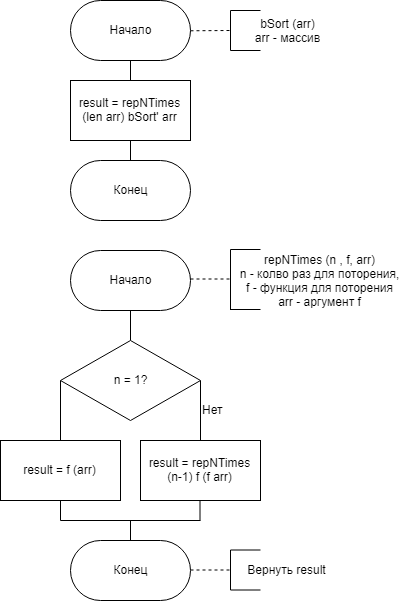
\includegraphics[scale=0.6]{bSort.png}
  \end{flushleft}
\end{minipage}
\hfill
\begin{minipage}{0.5\textwidth}
  \begin{flushright}
	\begin{center}
	bSort - это функция 'надстройка', едиснтвенная её задача - вызов функции repNTimes, следовательно
	\begin{equation}
	F_{bSort} = F_{repNTimes}
	\end{equation}
	~\\
	~\\
	~\\
	~\\
	~\\
	~\\
	~\\
	~\\
	~\\
	Максимальная глубина рекурсии функции repNTimes = N, что равно длине массива
	\begin{equation}
	F_{repNTimes} = N(2 + F_{bSort'}) - 1
	\end{equation}
	\end{center}
  \end{flushright}
\end{minipage}

\begin{minipage}{0.5\textwidth}
  \begin{flushleft}
	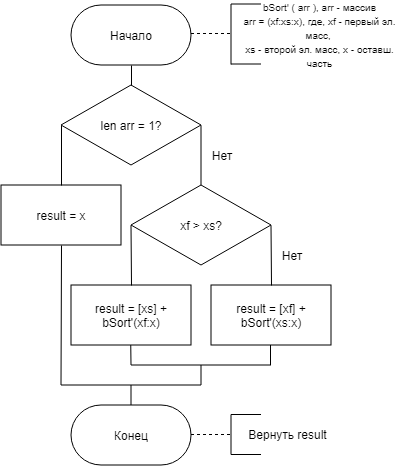
\includegraphics[scale=0.6]{bSort2.png}

	Рис 1. Схема алгоритма сортировки пузырьком.
  \end{flushleft}
\end{minipage}
\hfill
\begin{minipage}{0.5\textwidth}
  \begin{flushright}
	\begin{center}
		Максимальная глубина рекурсии bSort' так же равна N
		\begin{equation}
		F_{bSort'} = 3N - 1
		\end{equation}
	\end{center}
  \end{flushright}
\end{minipage}

\begin{center}
\textbf{Анализ трудоемкости:}
\begin{equation}
	F_{bSort} = F_{repNTimes} = N(2 + F_{bSort'}) - 1 = N(2 + 3N - 1) - 1 = N + 3N^2 - 1
\end{equation}

Для данной реализации алгоритма сортировки пузрьком, нет различий в трудоемкости при обратке обратно отсортированного массива, прямого или случайного.

Общая сложность алгоритма для всех случаев: {$O(N^2)$}
\end{center}








\chapter*{Список литературы}
\addcontentsline{toc}{chapter}{Список литературы}
\begin{enumerate} 
	\item В мире алгоритмов: Сортировка Вставками. [Электронный ресурс] Режим доступа: https://habr.com/ru/post/181271/ Последння дата обращения: 12.11.2019
\end{enumerate} 





























\end{document}